\chapter{Revisão Bibliográfica}      \label{Revisao Bibliografica}

Neste Capítulo, são apresentados os conceitos básicos da \textit{nanofotônica} (Seção \ref{Nanofotonica}), no que tange o desenvolvimento de dispositivos fotônicos e nanofotônicos, e os conceitos básicos do \textit{aprendizado de máquina} (Seção \ref{Machine Learning}), onde são introduzidos os conceitos de inteligência artificial e redes neurais profundas.

\section{Nanofotônica}      \label{Nanofotonica}

A nanofotônica é uma área da engenharia elétrica e engenharia ótica que visa o estudo da compreensão da luz nos materiais em escala nanométrica, o que certamente apresenta desafios para a ciência, ao mesmo tempo em que possibilita inovações tecnológicas. Esse estudo parte de várias frentes, como a investigação de novas interações óticas, de novos materiais, de técnicas de fabricação, bem como a exploração de estruturas orgânicas e inorgânicas, ou ainda, estruturas quimicamente fabricadas, como cristais fotônicos e pontos quânticos e plasmônicos \cite{ohtsu2008principles,shen2002nanophotonics}.

Nesse contexto, a crescente experiência da fusão da \textit{nanotecnologia} com a \textit{fotônica}, que são as duas principais tecnologias do século XXI, tem desempenhado um papel fundamental em muitos sistemas emergentes: seja em telecomunicações, como comutação óptica, espectroscopia, laser e fibra ótica \cite{Sumetsky2013Nanophotonics,6065798}; seja em aplicações médicas, como uma nova forma de diagnóstico e tratamento de câncer e imagens médicas \cite{Yunrun2021Application}; ou ainda, em energia renováveis, como em células fotovoltaicas de alta eficiência \cite{Albert2016Photovoltaic}. Este campo multidisciplinar também causou impacto na indústria, permitindo aos pesquisadores explorar novos horizontes em \textit{design}, na engenharia, na química, na física dos materiais, dentre outros \cite{kittel1996introduction,Joannopoulos:08:Book}.

O estudo das interações do fóton com a matéria em escalas incrivelmente pequenas, conhecidas como \textit{nanoestruturas}, tem como finalidade, sobretudo, o desenvolvimento de dispositivos e componentes em escala nanométrica para diversas funcionalidades, tendo em vista a capacidade de realizar muitas funções novas com base na interação eletromagnética local. Na nanofotônica, os conceitos tradicionais de \textit{interferência} e \textit{difração} (mecânica clássica) não são mais aplicáveis, mas substituídos por alguns novos conceitos \cite{band2013quantum,Joannopoulos:08:Book}. É nesse contexto de pesquisas que tem surgido nas últimas décadas o interesse e desenvolvimento de novos dispositivos nanofotônicos para operar como circuitos integrados em sistemas de telecomunmicações, especialmente, na região de interesse do \textit{terahertz} \cite{ghann2017terahertz,williams2007terahertz}.

A região terahertz (THz) do espectro eletromagnético, também chamada de \textit{THz GAP}, corresponde a uma faixa de comprimento de onda entre cerca de 3 mm e 30 $\mu m$ (ou ainda, de 100 GHz a 10 THz, em termos de frequência). Assim, como mostrado na Fig. \ref{fig: Therahertz}, em frequências mais baixas encontra-se o \textit{regime eletrônico} de radiação milimétrica ou de microondas, usado para aplicações em telecomunicações sem fio, como comunicação via satélite, rádio, etc. Para frequências mais altas, está o \textit{regime fotônico} (ou ainda, \textit{regime ótico}), onde dispositivos óticos ativos, como lasers de semicondutores e diodos emissores de luz, geram luz visível e infravermelha para transmissão em fibra óptica e armazenamento de dados \cite{ghann2017terahertz,fukunaga2009terahertz}.

\begin{figure}[H]
    \centering
    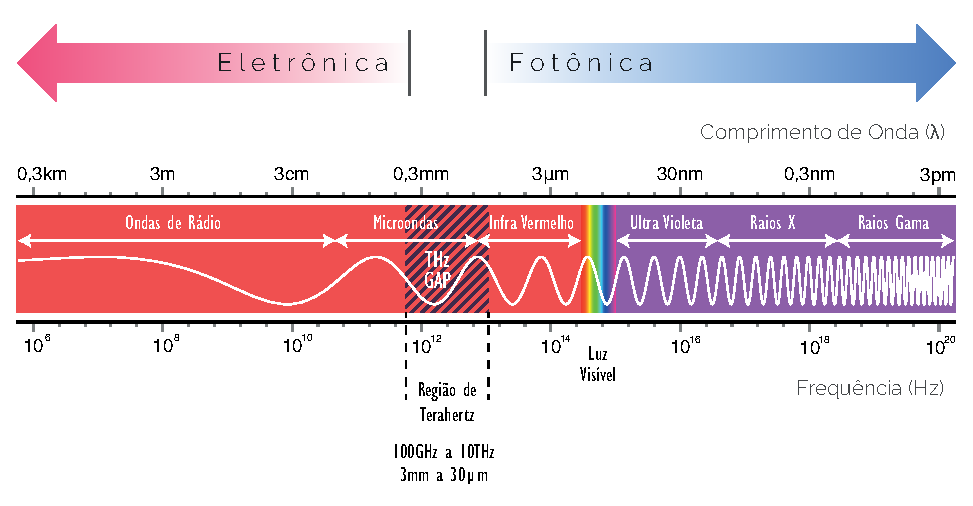
\includegraphics{04-Figuras/Therahertz.eps}
    \caption{Região de interesse em terahertz.} \par
    Fonte: do Autor.
    \label{fig: Therahertz}
\end{figure}

Entre esses dois mundos está a lacuna da tecnologia THz, região pouco explorada tecnologicamente em comparação com a maior parte do restante do espectro eletromagnético, pois, embora seja simples gerar e manipular micro-ondas e radiação infravermelha, ainda existem desafios tecnológicos a serem superados para a geração e detecção da radiação THz \cite{zhang2010introduction}. Os \textit{raios-T} (outro nome pelo qua a radiação THz é conhecida) têm aplicações potenciais em telecomunicações de última geração, incluindo as tecnologias de comunicação sem fio 6G e 7G \cite{Yang2020VisionOf6G}, em sistemas de segurança, exames médicos e até mesmo na análise de obras de arte \cite{fukunaga2007terahertz,fukunaga2009terahertz}.

Pelo fato da radiação THz ser do tipo \textit{não ionizante}, isso a torna segura para o uso em humanos, posto que possa penetrar em muitos materiais visualmente opacos. Isso a torna potencialmente útil na varredura de segurança de armas escondidas ou explosivos. A radiação terahertz facilmente pode ser absorvida pela água \cite{fukunaga2009terahertz}, entretanto, pode penetrar por alguns milímetros o tecido biológico, o que confere a capacidade para os pesquisadores estudarem os fundamentos da biologia celular e molecular \cite{tsurkan2013impact}.

\subsection{Nanoestruturas}

Alguns materiais 2D apresentam um potencial tecnológico extraordinário para a engenharia de dispositivos e componentes nanoeletrônicos e nanofotônicos, de forma que interagem muito bem com a radiação eletromagnética na faixa do terahertz. Alguns exemplos desses materiais (nanoestruturas) são o \textit{cristal fotônico} e o \textit{grafeno} \cite{Wang2018THz,Vitiello_2019}, mostrados na Fig. \ref{fig: PhotonicCrystalAndGraphene}.

\begin{figure}[H]
    \centering
    \includegraphics{04-Figuras/PhotonicCrystalAndGraphene.eps}
    \caption{Representação artística dos materiais. a) Cristal fotônico e seus arranjos dimensionais em 1D, 2D e 3D. b) Grafeno e sua estrutura hexagonal de um átomo de espessura.} \par
    Fonte: Isabelle Dumé (2021) \cite{Physicsworld2021Isabelle}; Elizabeth Gibney (2018) \cite{Nature2018Gibney} (Adaptado pelo Autor).
    \label{fig: PhotonicCrystalAndGraphene}
\end{figure}

Os \textit{cristais fotônicos} (do inglês: \textit{Photonic Crystals (PhC)}) são nanoestruturas projetadas para afetar o movimento dos fótons, definindo bandas de energia permitidas e proibidas \cite{ohtsu2008principles,shen2002nanophotonics}. Nesse sentido, os cristais fotônicos são compostos de nanoestruturas dielétricas e periódicas, com constante dielétrica alternada em uma, duas ou três dimensões para afetar a propagação de ondas eletromagnéticas dentro da estrutura. Como resultado dessa periodicidade, a transmissão da luz é absolutamente zero em certas faixas de frequência, o que é chamado de banda fotônica proibida (do inglês: \textit{Photonic Band Gap (PBG)}) \cite{yablonovitch1993photonic}.

Ao introduzir os defeitos (pequenas modificações) nessas estruturas periódicas, a periodicidade e, portanto, a integridade da \textit{banda fotônica proibida} é totalmente quebrada, o que permite controlar e manipular a luz \cite{yablonovitch1987inhibited} no material. Isso garante a localização da luz na região da banda fotônica proibida, o que possibilita ao desenvolvimento de dispositivos óticos baseados em cristais fotônicos \cite{john1987strong}.

Um outro exemplo de nanoestrutura muito estudada é o \textit{grafeno}, material 2D que mais vem sendo explorado nos últimos anos, sendo a substância mais fina já feita (contém apenas um átomo de espessura, como ilustrado na Fig. \ref{fig: PhotonicCrystalAndGraphene}.b)), o mais forte e o de maior mobilidade, demonstrado até agora. O grafeno explora uma condutividade térmica recorde que, combinada com sua qualidade cristalina e eletrônica excepcionalmente alta, permitiu abrir um novo paradigma da física da matéria condensada. Essas combinações de propriedades são bastantes peculiares do grafeno e não podem ser encontradas em nenhum outro material, ou ainda, sistema de materiais. Além disso, as propriedades óticas do grafeno, como o índice de refração, a absorção, velocidade de plasmon, dentre outras, podem ser ajustadas por meio de grade eletrostática ou pelo aumento do número de camadas. Isso implica que a permissividade do material pode ser alterada propositalmente, com a finalidade de que o grafeno possa se comportar como um material semicondutor, ou transparente, e até mesmo a propagação de plásmons em sua superfície \cite{Vitiello_2019}.

Portanto, as nanoestruturas são diversas e suas características físicas são bastantes estudadas para a fabricação de novos dispositivos, a exemplo de divisores de potência, chaves, circuladores, isoladores, dentre outros. Por conseguinte, metodologias computacionais têm sido amplamente empregadas para simular o comportamento funcional de estruturas nanofotônicas complexas que não possuem uma solução analítica.


\subsection{Divisores de Potência}

Um \textit{divisor de potência} divide um sinal de entrada em dois ou mais sinais de saída. Como ilustrado na Fig. \ref{fig: DividerDescription}, um dado dispositivo divisor de potência recebe um guia de onda externo incidente em uma porta (\textit{porta 1}) e o divide para as outras portas. Dependendo das características de projeto, pode ser interessante o isolamento alguma porta para a proteção de algumas partes do circuito (como ilustrado na Fig. \ref{fig: PhotonicCrystalAndGraphene}.b)). Também é interessante, enquanto característica de projeto, o isolamento contra possíveis reflexões do sinal para a própria porta excitada (\textit{porta 1}). 

\begin{figure}[H]
    \centering
    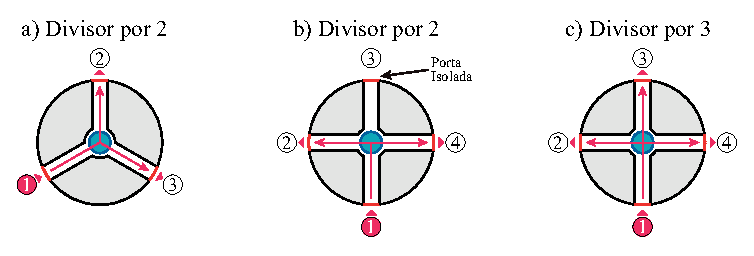
\includegraphics{04-Figuras/DividerDescription.eps}
    \caption{Ilustração de um dispositivo genérico divisor de potência. a) Divisor por 2. b) Divisor por 2 com uma porta isolada. a) Divisor por 3.} \par
    Fonte: do Autor.
    \label{fig: DividerDescription}
\end{figure}


\subsection{Circuladores}

Um \textit{circulador} é um dispositivo passivo, cuja a principal característica é fazer o sinal de entrada sair para a próxima porta. Por exemplo, como mostrado na Fig. \ref{fig: CirculatorDescription}, o sinal injetado na \textit{porta 1} interage com a cavidade ressonante central e segue para sair pela \textit{porta 2}, mas o contrário não acontece, isto é, o sinal injetado na \textit{porta 2} não retorna para a \textit{porta 1}. Essa características dos circuladores os tornam muito úteis para aplicações, por exemplo, que envolvem o acoplamento de transmissores e receptores que compartilham uma antenas comum, ao mesmo tempo em que isola o receptor do transmissor.

\begin{figure}[H]
    \centering
    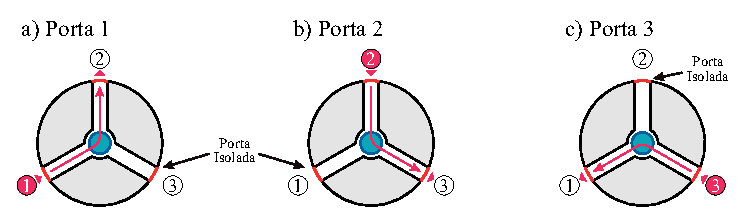
\includegraphics{04-Figuras/CirculatorDescription.eps}
    \caption{Ilustração de um dispositivo genérico circulador de três portas. a) Incidência na porta 1. b) Incidência na porta 2. c) Incidência na porta 3.} \par
    Fonte: do Autor.
    \label{fig: CirculatorDescription}
\end{figure}

Assim, os circuladores são descritos como componentes \textit{não recíprocos}, ou seja, o sinal na \textit{porta 1} sai predominantemente da \textit{porta 2} (Fig. \ref{fig: CirculatorDescription}.a)), o sinal na \textit{porta 2} sai pela \textit{porta 3} (Fig. \ref{fig: CirculatorDescription}.b)) e o sinal injetado pela \textit{porta 3} sai para a \textit{porta 1} (Fig. \ref{fig: CirculatorDescription}.c)). Em um dispositivo recíproco, a mesma fração do sinal que flui da \textit{porta 1} para a \textit{porta 2} ocorreria para o sinal fluindo na direção oposta, da \textit{porta 2} para a \textit{porta 1}.


\subsection{Parâmetros-S e Resposta em Frequência}

No estudo dos dispositivos nanofotônicos, uma maneira de avaliar o seu desempenho é através de sua resposta em frequência. Assim, pode-se mensurar os coeficientes de transmissão relacionados a cada porta. Por exemplo, para o circulador ilustrado na Fig. \ref{fig: CirculatorDescription}, a resposta em frequência está hipoteticamente ilustrada na Fig. \ref{fig: FrequencyResponseStudy}. Para as portas 1, 2 e 3 há três curvas sendo avaliada: curva de \textit{transmissão} (transmissão do sinal para a próxima porta), curva de \textit{isolamento} (isolamento do sinal para a porta que não seja a receptora) e curva de \textit{reflexão} (isolamento de relfexão do sinal para a própria porta emissora).

\begin{figure}[H]
    \centering
    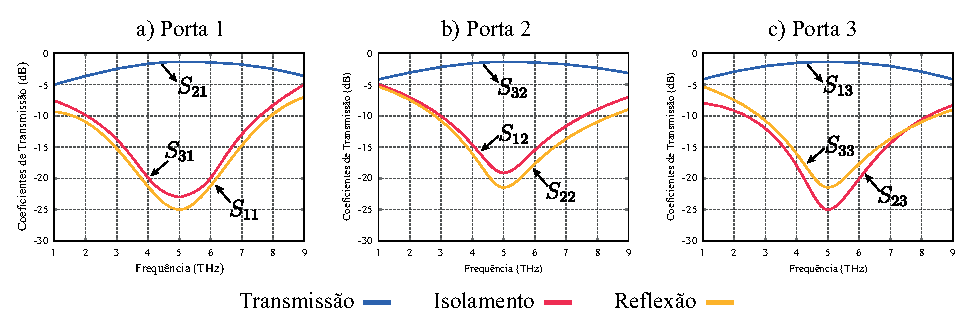
\includegraphics{04-Figuras/FrequencyResponseStudy.eps}
    \caption{Estudo da resposta em frequência para um dispositivo de três portas. a) Para a \textit{porta 1}. b) Para a \textit{porta 2}. c) Para a \textit{porta 3}} \par
    Fonte: do Autor.
    \label{fig: FrequencyResponseStudy}
\end{figure}

As aplicações em altas frequências tornaram-se cada vez mais predominantes com o avanço da eletrônica e da fotônica. Em circuitos de baixa frequência, por exemplo, parâmetros como tensão e corrente podem ser facilmente avaliados. Assim, os \textit{parâmetros-Y} e os \textit{parâmetros-Z} (admitância e impedância, respectivamente) podem ser usados para descrever uma rede. No entanto, para altas frequências, os \textit{parâmetros-S} são melhores aplicáveis para estudar um sistema multiporta, de forma que eles definem as ondas refletidas em termos das ondas incidentes nesses sistemas \cite{pupalaikis_2020}. Os parâmetros-S podem ser agrupados na forma matricial, conhecida como \textit{matriz de espalhamento}, onde a ordem $n$ da matriz $S$ representa o número de portas e cada elemento $S_{ij}$, representa o coeficiente de transmissão ou reflexão do sinal estudado entre as portas. Por exemplo, o elemento $S_{32}$ representa o coeficiente de transmissão avaliando um sinal da \textit{porta 2} para a \textit{porta 3}.

Para uma rede de três portas, como o dispositivo na representado na Fig. \ref{fig: CirculatorDescription}: os parâmetros $S_{11}$, $S_{22}$ e $S_{33}$ representam as perdas por reflexão das portas 1, 2 e 3, respectivamente; os parâmetros $S_{21}$, $S_{32}$ e $S_{13}$ representam os coeficientes de transmissão do sinal; e os parâmetros $S_{31}$, $S_{12}$ e $S_{23}$ representam os isolamentos.


\section{Aprendizado de Máquina}      \label{Machine Learning}

O aprendizado profundo (do inglês: \textit{Deep Learning (DL)}) é uma das áreas mais recentes em inteligência artificial, a qual envolve a aplicação de um subconjunto de ferramentas e técnicas de aprendizado de máquina (do inglês: \textit{Machine Lerarning (ML)}), permitindo que modelos computacionais compostos por múltiplas camadas de processamento aprendam a representação do dado em múltiplos níveis de abstração. Em termos práticos, isso possibilita aos sistemas aprender com dados, identificar padrões e tomar decisões com base no que foi aprendido \cite{goodfellow2016deep}. Esse processo possibilitou, sobretudo nos últimos anos, a revolução de muitas áreas da tecnologia, por exemplo, em carros autônomos \cite{al2017deep}, processamento de linguagem natural \cite{socher2013recursive}, reconhecimento facial e visão computacional \cite{krizhevsky2012imagenet}. Mas os avanços não são sentidos apenas pela indústria da tecnologia. As empresas e organizações também têm investido no uso de técnicas em aprendizado de máquina, no âmbito da \textit{ciência de dados}, para aumentar o lucro de seus negócios, ao mesmo tempo em que diminuem os custos de produção \cite{patil2015data,aggarwal2018neural}.

A inteligência artificial, propriamente dita, é apenas o produto final de um processo bem mais estruturado. Para fim de conceituação, a Fig. \ref{fig: AI_Map} esclarece a organização hierárquica das várias vertentes da inteligência artificial.

\begin{figure}[H]
    \centering
    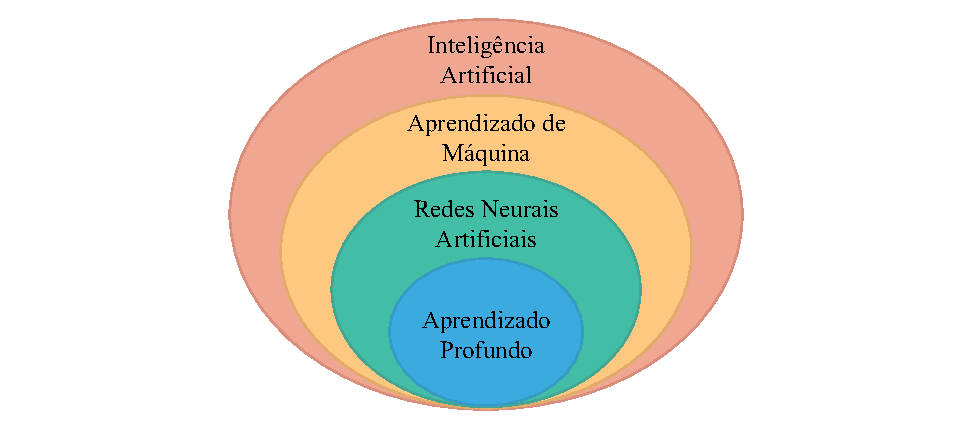
\includegraphics{04-Figuras/AI_Map.eps}
    \caption{Diagrama de Venn simplificado dos níveis hierárquicos da inteligência artificial.} \par
    Fonte: do Autor.
    \label{fig: AI_Map}
\end{figure}

As Redes Neurais Artificias (do inglês: \textit{Artificial Neural Network (ANN)}) são o começo das pesquisas em inteligência artificial. Assim, elas são técnicas computacionais que partem de uma modelagem matemática inspiradas na estrutura neural biológica dos organismos inteligentes. Estruturas mais complexas das ANNs são as \textit{Redes Neurais Profundas} (do inglês: \textit{Deep Neural Networks (DNN)}). Elas são versáteis, poderosas e escaláveis, tornando-as ideais para lidar com tarefas de aprendizado de máquina grandes e altamente complexas, envolvendo problemas multivariáveis \cite{lecun2015deep}. Os exemplos de aplicações estão muito presentes no dia-a-dia, como usados pelo \textit{Google}: para a classificação de bilhões de imagens no mecanismos de pesquisa \textit{Google Imagens}; para o melhoramento de tradução entre diversos idiomas do \textit{Google Tradutor}; para o sistema de recomendação de vídeos do \textit{Youtube} \cite{castelvecchi2016deep}.


\subsection{Redes Neurais Artificiais}

As Redes Neurais Artificiais são uma das estruturas que compõe a base da inteligência artificial e tem raízes em disciplinas como neurociência, matemática, estatística, física, ciência da computação e engenharia. Suas aplicações podem ser encontradas em campos tão diversos quanto modelagem, análise de séries temporais, reconhecimento de padrões, processamento de sinais e controle. Elas são uma modelagem matemática-computacional dos neurônios biológicos humanos. 

O estudo sobre RNAs eixste há bastante tempo. Elas foram aboradas pela primeira vez em 1943 pelo neurofisiologista Warren McCulloch e pelo matemático Walter Pitts. Foi através do artigo \textit{A Logical Calculus of the Ideas Immanent in Nervous Activity} \cite{mcculloch1943logical} que McCulloch e Pitts apresentaram um modelo computacional simplificado de como os neurônios biológicos podem trabalhar juntos em cérebros de animais para realizar cálculos complexos usando lógica proposicional. Esta foi a primeira arquitetura de rede neural artificial.


\subsection{Fundamentos Biológicos}

Antes de discutirmos os neurônios artificiais propriamente ditos, é interessante pontuar algumas características de um neurônio biológico (representado na Fig. \ref{fig: Neuron}).

\begin{figure}[H]
    \centering
    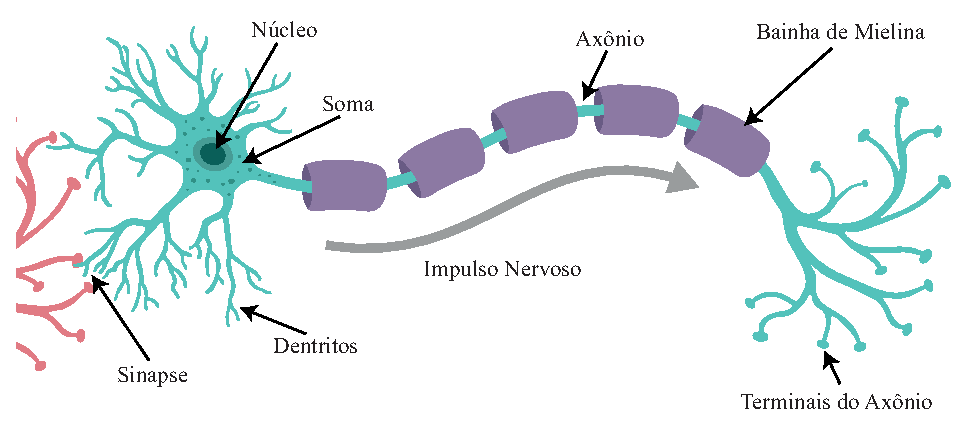
\includegraphics[width=\textwidth]{04-Figuras/Neuron.eps}
    \caption{Neurônio biológico.} \par
    Fonte: do Autor.
    \label{fig: Neuron}
\end{figure}

O neurônio é uma célula de aparência bastante característica encontrada, principalmente, em córtex cerebral de animais, composta por um corpo celular que contém o \textit{núcleo} e a maioria dos componentes complexos da célula, e muitas extensões ramificadas chamadas \textit{dendritos}, além de uma extensão longa chamada de \textit{axônio}. O comprimento do axônio pode ser apenas algumas vezes maior do que o corpo celular ou até dezenas de milhares de vezes maior. Perto de sua extremidade, o axônio se divide em muitos ramos chamados \textit{terminais}, e na ponta desses ramos estão estruturas minúsculas chamadas de \textit{sinapses}, que estão conectadas aos dendritos de outros neurônios, e assim por diante, formando uma \textit{rede neural biológica}. Os neurônios biológicos recebem impulsos elétricos curtos (chamados de \textit{sinais}) de outros neurônios por meio dessas sinapses. Quando um neurônio recebe um número suficiente de sinais de outros neurônios em alguns milissegundos, então, ele dispara seus próprios sinais \cite{gerstner2002spiking,dayan2001theoretical}.

Individualmente, os neurônios biológicos parecem se comportar de uma forma bastante simples, entretanto, eles são organizados em uma estrutura em circuito, formando uma vasta rede de bilhões de neurônios, onde cada neurônio normalmente está conectado a outros milhares de neurônios. A arquitetura das redes neurais biológicas é constantemente objeto de pesquisas. Algumas partes do cérebro foram mapeadas por \textit{Santiago Ramon y Cajal (1899)} e, como mostrado na Fig. \ref{fig: Cajal_cortex_drawings}, os neurônios costumam ser organizados em camadas consecutivas.

\begin{figure}[H]
    \centering
    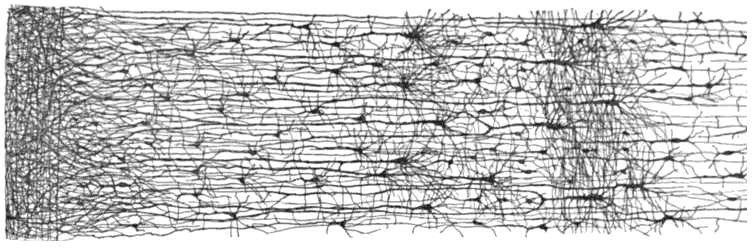
\includegraphics[width=\textwidth]{04-Figuras/Cajal_cortex_drawings.png}
    \caption{Desenho de laminação cortical de Santiago Ramon y Cajal mostrando uma seção transversal da rede neural biológica (córtex humano) com os neurônios dispostos em múltiplas camadas.} \par
    Fonte: Santiago Ramon y Cajal (1899) \cite{y1899comparative}.
    \label{fig: Cajal_cortex_drawings}
\end{figure}


\subsection{Neurônio Artificial}

Warren McCulloch e Walter Pitts propuseram um modelo muito simples do neurônio biológico, que mais tarde ficou conhecido como um \textit{neurônio artificial} \cite{mcculloch1943logical}: é constituído de uma ou mais entradas binárias (\textit{nível lógico alto / nível lógico baixo}) e uma saída binária, de forma que neurônio artificial simplesmente ativa sua saída quando mais de um certo número de suas entradas estão ativas. Décadas de desenvolvimento e contribuição de vários pesquisadores, por fim, resultaram no modelo de neurônio artificial usado atualmente, conhecido como \textit{perceptron} \cite{aggarwal2018neural,haykin2007redes}.

Um neurônio artificial recebe em sua entrada sinais originários de outros neurônios. Essas conexões (\textit{sinapses}) são ponderadas por elementos chamados de \textit{pesos sinápticos}. Nessa linha, as entradas do neurônio podem ser \textit{excitatórias ou \textit{inibitórias}}. Assim, um neurônio artificial só poderá passar um sinal de saída para a próxima camada, caso suas entradas somam um valor acima de um determinado valor limite, isto é, necessitam atingir um limiar de ativação (\textit{função de ativação}) para o sinal ser propagado adiante. A Fig. \ref{fig: ArtificialNeuronModel} mostra um diagrama de blocos da representação matemática de um neurônio artificial perceptron.

\begin{figure}[H]
    \centering
    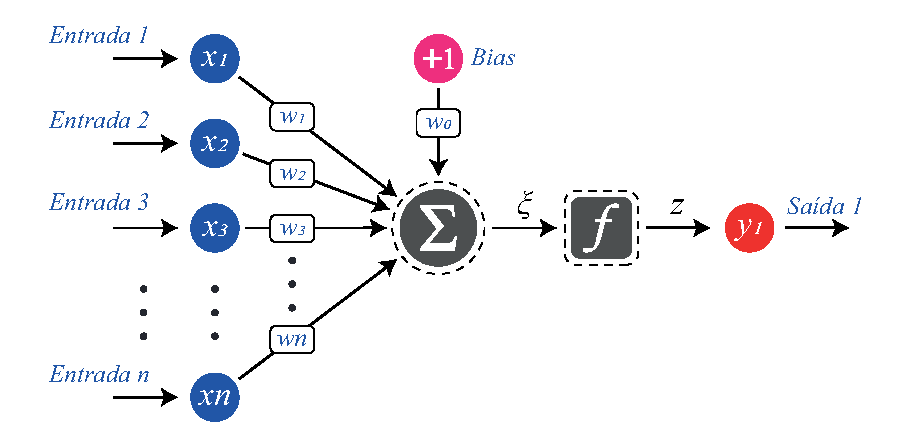
\includegraphics{04-Figuras/ArtificialNeuronModel.eps}
    \caption{Diagrama de blocos de um neurônio artificial.} \par
    Fonte: do Autor.
    \label{fig: ArtificialNeuronModel}
\end{figure}

Na Fig. \ref{fig: ArtificialNeuronModel}, $x_{1}, x_{2}, \cdots, x_{n}$ são as entradas; $w_{1}, w_{2}, \cdots, w_{n}$ são os pesos sinápticos; $\varphi(\cdot)$ é a função de ativação; e, por fim, $y$ é o sinal de saída do neurônio. O somatório de todas as entradas do neurônio, ponderadas de pesos sinápticos, posteriormente submetidos a uma função de ativação, dão origem ao sinal de saída do neurônio. Nesse processo, o \textit{Bias} (definido por $b$) é uma estrutura invariante de valor $1$, ponderada de um peso $w_{0}$. Em termos práticos, o \textit{Bias} permite que o neurônio apresente uma saída não nula, ainda que todas as entradas sejam nulas \cite{haykin2007redes,aggarwal2018neural}. Matematicamente, um neurônio artificial $j$ é modelado conforme as Eqs. \ref{eq: Neuron} e \ref{eq: Neuron phi}.

\begin{equation}    \label{eq: Neuron}
    v_{j} = \sum_{i=1}^{n}w_{ij}\cdot x_{ij} + b_{j}
\end{equation}

Uma sinapse $i$ causa um efeito pós-sináptico descrito por $w_{i}x_{i}$. A sinapse será \textit{excitatória} se $w_{i} > 0$ e \textit{inibitória} se $w_{i} < 0$. A Eq. \ref{eq: Neuron phi} mostra a saída do neurônio.

\begin{equation}    \label{eq: Neuron phi}
    y_{j} = \varphi(v_{j})
\end{equation}


\subsection{Função de Ativação}

A função de ativação $\varphi(\cdot)$ é uma transformação que será aplicada às entradas (ponderadas) antes do sinal ser enviado para a próxima camada de neurônios, sendo essencial para determinar a saída desse neurônio, pois decidirá se o neurônio deve ser ativado ou não. A escolha da função de ativação tem um grande impacto na capacidade e no desempenho da rede neural, e diferentes funções de ativação podem ser usadas em diferentes partes do modelo. Existem muitos tipos de funções de ativação usadas em redes neurais, algumas das quais estão ilustradas na Fig. \ref{fig: NetworkActvationFunction}.

\begin{figure}[H]
    \centering
    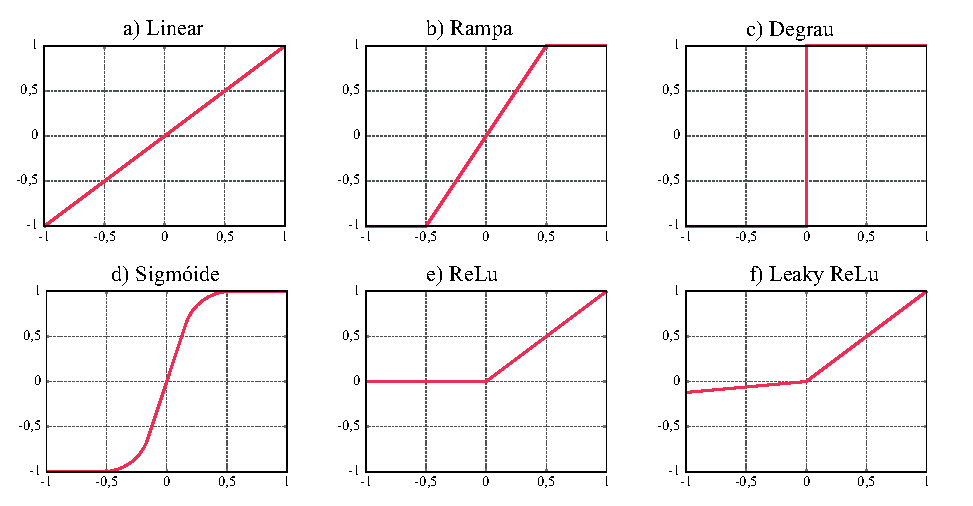
\includegraphics{04-Figuras/NetworkActvationFunction.eps}
    \caption{Funções de ativação. a) Linear. b) Linear. c) Linear. d) Linear. e) ReLu. f) Leaky ReLu.} \par
    Fonte: do Autor.
    \label{fig: NetworkActvationFunction}
\end{figure}

A escolha da função de ativação é uma parte crítica do projeto da rede neural e a sua escolha é feita de acordo com a finalidade de previsão na saída do neurônio. Por exemplo, se a saída for um valor real, então o mais adequado é usar uma função de ativação \textit{Linear} (Eq. \ref{eq: ActFunc Linear}), já que produz uma saída contínua e o algoritmo resultante torna-se o mesmo que uma regressão de mínimos quadrados \cite{aggarwal2018neural}. Quando se deseja produzir uma saída contínua apenas em uma dada faixa de valores, o mais apropriado é a função \textit{rampa} (Eq. \ref{eq: ActFunc HardTanh}) (ou ainda, \textit{hard tanh}). A função \textit{Degrau} (Eq. \ref{eq: ActFunc Step}) é usada para representar uma saída de estados binários. A função \textit{Sigmóide} (Eq. \ref{eq: ActFunc Sigmoide}) é mais adequada para previsões que envolvam uma probabilidade de classes binárias.

Por fim, a função \textit{ReLu} (do inglês: \textit{Rectified Linear Unit}) é uma das funções de ativação mais utilizadas atualmente, principalmente em \textit{redes neurais convolucionais}\footnote{Classe de rede neural artificial do tipo \textit{feedforward}, muito utilizada em processamento e análise de imagens digitais.} ou \textit{aprendizado profundo} \cite{agarap2018deep,lin2018research}. Assim, a função \textit{ReLu} (Eq. \ref{eq: ActFunc ReLu}) é retificada pela metade (na parte inferior), de forma que valores negativos tornam-se zero imediatamente, o que acaba gerando um problema por não mapear os valores negativos de forma adequada. Uma função que tenta resolver esse problema é a \textit{Leaky ReLu} (Eq. \ref{eq: ActFunc LeakyReLu}), que é um tipo de função de ativação baseada em \textit{ReLU}, mas tem uma pequena inclinação para valores negativos ao invés de retificá-los \cite{aggarwal2018neural}.

\begin{equation}    \label{eq: ActFunc Linear}
    \varphi(x) = x
\end{equation}

\begin{equation}    \label{eq: ActFunc HardTanh}
    \varphi(x) =
    \begin{cases}
    + \lambda, & \text{ se } x \geq + \lambda,\\
    x,         & \text{ se } \left | x \right | < + \lambda,\\
    - \lambda, & \text{ se } \left | x \right | \leq - \lambda.
    \end{cases}
\end{equation}

\begin{equation}    \label{eq: ActFunc Step}
    \varphi(x) =
    \begin{cases}
    +1, & \text{ se } x \geq 0,\\
    -1, & \text{ se } x < 0.
    \end{cases}
\end{equation}

\begin{equation}    \label{eq: ActFunc Sigmoide}
    \varphi(x) = \frac{1}{1 + e^{-x}}
\end{equation}

%\begin{equation}    \label{eq: ActFunc ReLu}
%    f(x) = max(0,x)
%\end{equation}

\begin{equation}    \label{eq: ActFunc ReLu}
    \varphi(x) =
    \begin{cases}
    x, & \text{ se } x \geq 0,\\
    0, & \text{ se } x < 0.
    \end{cases}
\end{equation}

\begin{equation}    \label{eq: ActFunc LeakyReLu}
    \varphi(x) =
    \begin{cases}
    x,         & \text{ se } x \geq 0,\\
    a \cdot x, & \text{ se } x < 0.
    \end{cases}
\end{equation}

Normalmente, todas as camadas ocultas usam a mesma função de ativação. A camada de saída normalmente usará uma função de ativação diferente das camadas ocultas e sua escolha depende muito do tipo de previsão exigida pelo modelo.


\subsection{Perceptron Multicamadas}

A arquitetura de uma rede neural é determinada pela forma com a qual os seus neurônios e camadas estão conectados \cite{haykin2007redes}. O modelo \textit{perceptron} de camada única (mostrado na Fig. \ref{fig: ArtificialNeuronModel}) não pode produzir o tipo de desempenho que se espera de uma arquitetura de rede neural moderna, pois é limitado para a resolução de problemas linearmente separáveis, não sendo capaz de aproximar as relações complexas de entrada e saída que ocorrem em cenários de processamento de sinal da vida real \cite{aggarwal2018neural,haykin2007redes}.

Enquanto que em uma rede de única camada, as entradas são diretamente mapeadas para a saída através de uma transformação da função de ativação, nas redes neurais com múltiplas camadas, as camadas de \textit{entrada} e \textit{saída} são separadas por um grupo de camadas \textit{intermediárias}. Esse modelo descrito é uma classe de \textit{rede feedforward} conhecida como \textit{Muitilayer Perceptron (MLP)} \cite{aggarwal2018neural,haykin2007redes}.

\begin{figure}[H]
    \centering
    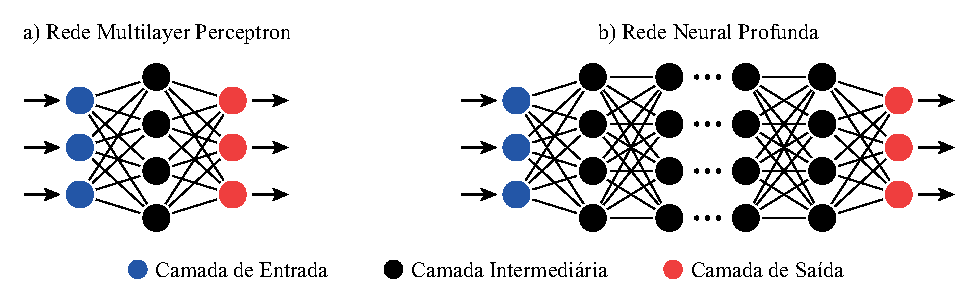
\includegraphics{04-Figuras/NeuralNetworkAndDeepLearning.eps}
    \caption{Redes \textit{Muitilayer Perceptron (MLP)}. a) Rede MLP padrão. b) Rede neural profunda.} \par
    Fonte: do Autor.
    \label{fig: NeuralNetworkAndDeepLearning}
\end{figure}

A Fig. \ref{fig: NeuralNetworkAndDeepLearning} mostra duas arquiteturas de redes \textit{feedforward}, sendo a Fig. \ref{fig: NeuralNetworkAndDeepLearning}.a) um modelo padrão, com uma única camada intermediária e a Fig. \ref{fig: NeuralNetworkAndDeepLearning}.b) uma rede com várias camadas intermediárias, caracterizando uma Rede Neural Profunda (do inglês: \textit{Deep Neural Network (DNN)}). 

No geral, duas classes de redes são bastante populares e estudadas: as \textit{redes de alimentação para frente} (do inglês: \textit{feedforward}\footnote{Neste documento, será utilizado o termo \textit{feedforward} para citar as \textit{redes de alimentação para frente}.}) e as \textit{redes recorrentes}, como mostradas na Fig. \ref{fig: NeuralNetworkFeedforwardAndRecurrent}.

\begin{figure}[H]
    \centering
    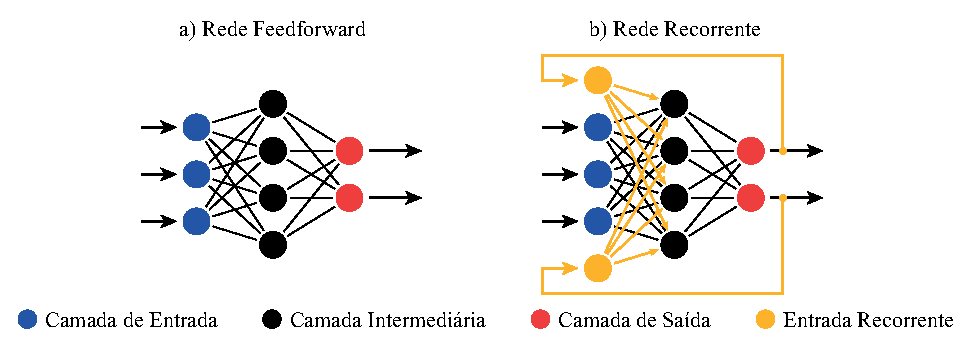
\includegraphics{04-Figuras/NeuralNetworkFeedforwardAndRecurrent.eps}
    \caption{Principais classes de redes neurais. a) Rede feedforward. b) Rede recorrente.} \par
    Fonte: do Autor.
    \label{fig: NeuralNetworkFeedforwardAndRecurrent}
\end{figure}

Nas redes \textit{feedforward} há um fluxo de informações unidirecional, fluindo das entradas da rede para a saída. Para as redes \textit{recorrentes}, por outro lado, há uma realimentação da saída nas próprias entradas. Uma característica interessante das redes recorrentes é que elas podem suportar memória de curto prazo \cite{russell2020artificial}.


\subsection{Algoritmos e Processos de Aprendizagem}

O principal objetivo de uma rede neural é aprender a partir do ambiente\footnote{O termo \textit{ambiente} indica a situação para a qual uma rede neural artificial está submetida a aprender.} e de melhorar o seu desempenho através de um processo de aprendizagem \cite{haykin2007redes}. Esse processo segue alguns passos: primeiro, a rede neural é estimulada pelo ambiente; após esse estímulo, a rede neural sofre modificações nos seus parâmetros internos (pesos sinápticos); por fim, a rede neural agora responde ao ambiente de uma forma nova, devido às modificações ocorridas na sua estrutura interna. Assim, uma rede neural irá sintetizar um modelo de aprendizado, a partir de dados do ambiente, através de um processo iterativo de ajustes dos pesos sinápticos, chamado de \textit{treinamento} \cite{haykin2007redes,russell2020artificial}.

Outra abordagem é como uma rede neural se relaciona com o seu ambiente, conceito esse que descreve um \textit{paradigma de aprendizagem} \cite{haykin2007redes}, sendo eles \textit{Aprendizado Supervisionado}, \textit{Aprendizado Não Supervisionado} e \textit{Aprendizado Por Reforço}.

No \textit{aprendizado supervisionado}, as entradas e as saídas (banco de dados) são fornecidos por um \textit{supervisor} (professor), como mostrado na Fig. \ref{fig: NeuralNetworkSupervisedLearning}. O algoritmo faz previsões iterativamente sobre os dados de treinamento e é corrigido pelo professor. O aprendizado para quando o algoritmo atinge um nível aceitável de desempenho \cite{haykin2007redes}.

\begin{figure}[H]
    \centering
    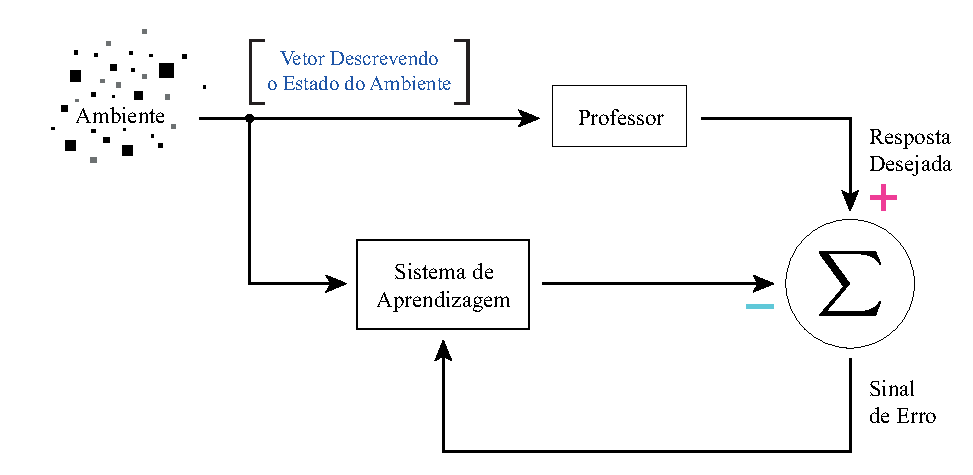
\includegraphics{04-Figuras/NeuralNetworkSupervisedLearning.eps}
    \caption{Aprendizado Supervisionado.} \par
    Fonte: do Autor.
    \label{fig: NeuralNetworkSupervisedLearning}
\end{figure}

No aprendizado \textit{não supervisionado}, a rede neural é posta ao ambiente, de forma que apenas dados de entrada são fornecidos (não há professor para acompanhar o processo de treinamento). Nesse sentido, a rede irá se auto organizar em relação às particularidades e características do conjunto de amostras que representam o ambiente \cite{haykin2007redes}.

No \textit{aprendizado por reforço}, a própria rede aprende a atingir um objetivo a partir do que o ambiente lhe oferece. Assim, para que a máquina faça o que o programador quer (objetivo), a inteligência artificial recebe recompensas ou penalidades pelas ações que realiza (reforço). Seu objetivo é maximizar a recompensa total \cite{haykin2007redes}.

Os algoritmos de aprendizado usam um conjunto de regras bem definidas, chamadas de \textit{regras de aprendizagem}, para determinar maneira como a atualização dos pesos devem ocorrer. Os exemplos de regras mais comuns são a \textit{regra delta}, a \textit{regra de Hebb}, \textit{regra perceptron} e a \textit{regra de aprendizado competitivo}.

Muitos algoritmos de otimização (chamados de \textit{otimizadores}) foram desenvolvidos, sendo alguns dos otimizadores mais usados são: Adagrad, Adadelta, Adam, Nadam, SGD e RMSprop. Cada um deles irá usar uma regra de aprendizagem, no contexto dos paradigmas de aprendiagem, para atualizar os pesos sinápticos de uma rede neural. Assim, os otimizadores atualizam os parâmetros de peso para minimizar a função custo por um método iterativo do \textit{gradiente descedente} \cite{haykin2007redes,bottou2010large,geron2019hands}. A função custo atua como um guia para o otimizador, dizendo se ele está se movendo na direção certa para chegar ao mínimo (local ou global), como ilustrado na Fig. \ref{fig: GradientDescent}.

\begin{figure}[H]
    \centering
    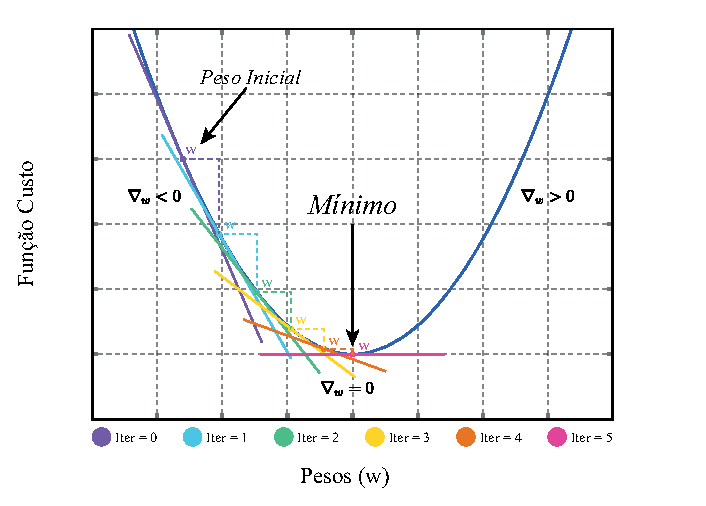
\includegraphics{04-Figuras/GradientDescent.eps}
    \caption{Descida do gradiente.} \par
    Fonte: do Autor.
    \label{fig: GradientDescent}
\end{figure}

A frequência de atualização dos pesos sinápticos de uma rede neural é outro fator que deve ser avaliado. Durante o treinamento, a rede neural será exposta às instâncias do banco de dados (cada amostra do banco de dados). O tamanho do lote (\textit{Batch}) é um hiperparâmetro que define o número de amostras a serem trabalhadas antes de atualizar os parâmetros do modelo interno. Há duas abordagens de como ocorre a correção dos pesos:

\begin{itemize}
    \item \textbf{Modo Padrão:} a correção dos pesos sinápticos ocorre a cada apresentação de partes (batch) bem definidas do banco de dados (ver Fig. \ref{fig: BatchEpoch}).
    \item \textbf{Modo Batch:} neste modo, apenas uma correção é feita por época. Desta maneira, o número de iterações e épocas são equivalentes (ver Fig. \ref{fig: BatchEpoch}).
\end{itemize}

Tomando um exemplo prático. Um banco de dados contendo 20 instâncias (ou amostras), supondo que o tamanho de lote (\textit{batch}) escolhido foi de 4 e o número de épocas foi de 1. Isso significa que o banco de dados será dividido em 5 lotes, cada um contendo 4 amostras. Desta forma, os pesos do modelo serão atualizados após cada lote de 4 amostras. Assim, uma época terá 5 atualizações do modelo, ou ainda, 5 iterações. Uma \textit{época} refere-se a todas as amostras do banco de dados iteradas (pesos atualizados) uma vez, como mostra a Fig. \ref{fig: BatchEpoch}.

\begin{figure}[H]
    \centering
    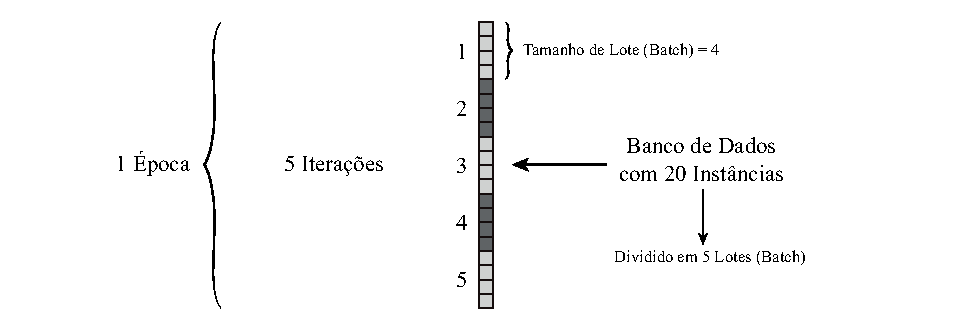
\includegraphics{04-Figuras/BatchEpoch.eps}
    \caption{Divisão das amostras do banco de dados.} \par
    Fonte: do Autor.
    \label{fig: BatchEpoch}
\end{figure}

Com 100 épocas, o modelo será exposto por todas as amostras do banco de dados 100 vezes, processo que levará 500 iterações.


\subsection{Algoritmo Backpropagation}

O algoritmo \textit{backpropagation} é o mais importante da história das redes neurais modernas e da aprendizagem profunda. O seu objetivo é otimizar os pesos sinápticos, através da retropropagação do erro, para que a rede neural possa aprender a mapear corretamente a relação entre os dados de entrada para com os dados de saída. O \textit{backpropagation} é mais utilizado para o treinamento de redes \textit{feedforward} \cite{haykin2007redes}, processo no qual envolve duas etapas básicas:

\begin{itemize}
    \item O \textbf{passo para frente (\textit{forward pass})}: nesse primeiro passo, um padrão de atividades do ambiente (vetor de entrada) é propagado através da rede, e as previsões de saída são obtidas. Nesse contexto, os pesos sinápticos da rede são todos fixos (são iniciados de forma randômica).
    \item O \textbf{passo para trás (\textit{backward pass})}: Nessa etapa, é calculado o gradiente da função custo na camada final da rede, de forma que esse gradiente é utilizado para aplicar recursivamente a regra da cadeia na função custo a fim de atualizar os pesos da rede.
\end{itemize}

Assim, o algoritmo \textit{backpropagation} define erros no desempenho de cada neurônio, possibilitando os ajustes dos pesos sinápticos. Sendo $y$ a saída esperada e $\hat{y}$ a saída obtida pela rede, a função de erro (custo) é definida pelo erro médio quadrático (\textit{Mean Squared Error (MSE)}), mostrado pela Eq. \ref{eq: Funcao de erro}.

\begin{equation}    \label{eq: Funcao de erro}
    E({y,\hat{y}}) = \frac{1}{2}\sum_{i=1}^{n}\left ( y_{i} - \hat{y}_{i} \right )^{2}
\end{equation}

O algoritmo, então, calcula a derivada parcial da função a ser minimizada em relação ao respectivo peso, como mostrado na Eq. \ref{eq: Back Parcial 1}.

\begin{equation}    \label{eq: Back Parcial 1}
    \frac{\partial E(y_{i},\hat{y}_{i})}{\partial w_{ij}} = \frac{\partial E(y_{i},\hat{y}_{i})}{\partial \hat{y}} \frac{\partial \hat{y}}{\partial v_{j}} \frac{\partial v_{j}}{\partial w_{ij}}
\end{equation}

\noindent
onde $v_{j}$ é a saída do somador do neurônio $j$. Considerando uma função de ativação genérica $\varphi(v_{j})$:

\begin{equation}
    \frac{\partial E(y_{i},\hat{y}_{i})}{\partial w_{ij}} = - \left ( y_{i} - \hat{y}_{i} \right ) \varphi^{,}(v_{j}) \frac{\partial v_{j}}{\partial w_{ij}}
\end{equation}

\noindent
onde:

\begin{equation}
    \frac{\partial v_{j}}{\partial w_{ij}} = \frac{\partial (x_{1}w_{1} + x_{2}w_{2} + \cdots + x_{nj}w_{nj})}{\partial w_{i}} = x_{nj}
\end{equation}

\noindent
portanto:

\begin{equation}    \label{eq: Backpropagation Final}
    \frac{\partial E(y_{i},\hat{y}_{i})}{\partial w_{ij}} = - \left ( y_{i} - \hat{y}_{i} \right ) \varphi^{,}(v_{j}) x_{i}
\end{equation}

A Eq. \ref{eq: Backpropagation Final} mostra o cáculo do gradiente da função custo. Por fim, na etapa de retropropagação, a atualização de cada um dos pesos $w_{ij}$ pesos sinápticos é feita pela \textit{regra delta}, definida pela Eq. \ref{eq: peso W}.

\begin{equation}    \label{eq: peso W}
    w_{ij}^{+} = w_{ij} - \eta\frac{\partial E(y_{i},\hat{y}_{i})}{\partial w_{ij}},
\end{equation}

\noindent
onde $w^{+}_{ij}$ é o novo peso sináptico, $w_{ij}$ é o peso atual e $\eta$ é a taxa de aprendizagem (\textit{learning rate}). No aprendizado de máquina, a regra delta (ver Eq. \ref{eq: Regra Delta}) é uma regra de aprendizado de gradiente descedente para atualizar os pesos sinápticos dos neurônios artificiais. Assim, em cada iteração, a regra de atualização dos pesos é executada, onde será definido o próximo ponto que fará a descida do gradiente, um ponto que está mais abaixo na função, rumo ao mínimo.

\begin{equation}    \label{eq: Regra Delta}
    \left({\begin{tabular}{c}
    Correção \\
    de peso\\
    $\Delta w(n)$
    \end{tabular}}\right)
    =
    \left({\begin{tabular}{c}
    Parâmetro da taxa\\
    de aprendizagem\\
    $\eta$
    \end{tabular}}\right)
    \cdot
    \left({\begin{tabular}{c}
    Gradiente \\
    local\\
    $\delta(n)$
    \end{tabular}}\right)
    \cdot
    \left({\begin{tabular}{c}
    Sinal de entrada\\
    do neurônio j\\
    $y(n)$
    \end{tabular}}\right)
\end{equation}

A taxa de aprendizagem é introduzida como uma constante (geralmente muito pequena), a fim de forçar o peso a ser atualizado de forma suave e lenta, por exemplo, para evitar grandes passos e comportamento caótico \cite{geron2019hands,haykin2007redes}. Quando essa taxa $\eta$ é muito grande, os passos de convergência são grandes também e isso pode ocasionar em \textit{pular o mínimo} várias vezes sem nunca convergir. Quando $\eta$ é muito pequeno, os passos de convergência também são pequenos, o que fará o algoritmo convergir, entretanto, poderá levar muito tempo para isso acontecer.